\section{Entrega parcial 2}

\subsection{Diseño conceptual y codificación de 2 (dos) niveles de anidación de colecciones de objetos}

\begin{figure}[h]
    \centering
    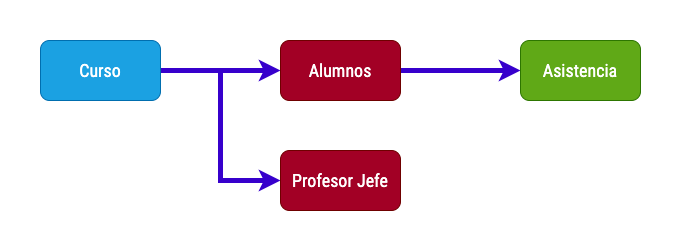
\includegraphics[width=0.9\textwidth]{contents/img/img4}
    \caption{Anidación de colecciones de objetos}
    \label{fig:img4}
\end{figure}

Como podemos ver en la \hyperref[fig:img4]{imagen}, el proyecto está planificado para contener la colección de cursos, la que a su vez contiene un \textbf{HashMap} de \textit{Alumnos} y el \textit{Profesor jefe} a cargo. En cuanto a la asistencia, cada \textit{Alumno} contendrá un \textbf{HashMap} con su asistencia personal.

\subsection{Diseño conceptual y codificación de 2 (dos) clases que utilicen sobrecarga de métodos}

\begin{figure}[h]
    \centering
    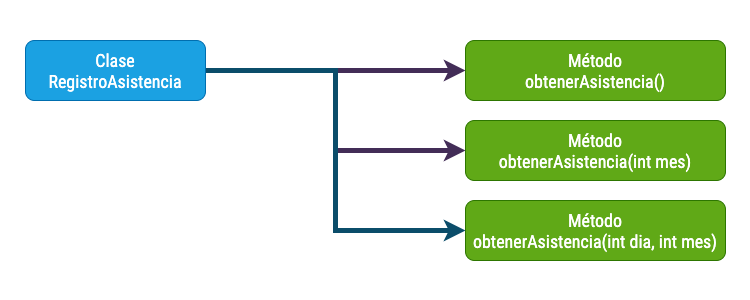
\includegraphics[width=0.9\textwidth]{contents/img/img5}
    \caption{Sobrecarga de métodos: Clase RegistroAsistencia}
    \label{fig:img5}
\end{figure}

Los métodos \mintinline{java}{obtenerAsistencia} de la clase \textbf{RegistroAsistencia} obtienen los datos de asistencia del alumno con los siguientes retornos:

\begin{itemize}
    \item \mintinline{java}{public float obtenerAsistencia()}: Retorna el promedio de asistencia del alumno, calculado al día de realizada la consulta.
    \item \mintinline{java}{public float obtenerAsistencia(int mes)}: Retorna el promedio de asistencia del alumno, del mes especificado como parámetro.
    \item \mintinline{java}{public float obtenerAsistencia(int dia, int mes)}: Retorna el valor de asistencia del alumno en el día y mes especificados como parámetros.
\end{itemize}

\begin{figure}[h]
    \centering
    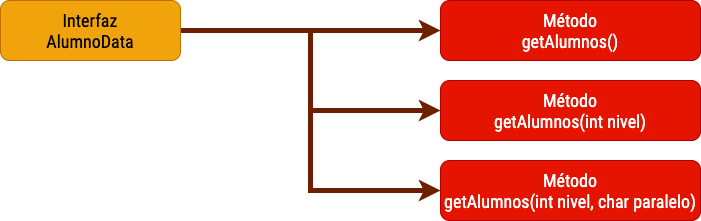
\includegraphics[width=0.9\textwidth]{contents/img/img6}
    \caption{Sobrecarga de métodos: Interfaz AlumnoData}
    \label{fig:img6}
\end{figure}

Los métodos \mintinline{java}{getAlumnos} de la interfaz \textbf{AlumnoData} obtienen los datos de los alumnos con los siguientes retornos:

\begin{itemize}
    \item \mintinline{java}{public Map<String, Alumno> getAlumnos()}: Retorna un HashMap con todos los alumnos almacenados.
    \item \mintinline{java}{public Map<String, Alumno> getAlumnos(int nivel)}: Retorna un HashMap con todos los alumnos del nivel especificado como parámetro.
    \item \mintinline{java}{public Map<String, Alumno> getAlumnos(int nivel, char paralelo)}: Retorna un HashMap con todos los alumnos del curso especificado (nivel y paralelo).
\end{itemize}

\subsection{Diseño conceptual y codificación de al menos 1 clase mapa del JCF}

Cada \textbf{Curso} debe manejar un número indeterminado de \textbf{Alumnos}, y su recorrido debe ser lo más eficiente posible a la hora de buscar un alumno específico, dado que el programa debe manejar los registros de asistencia, que están anidados en cada alumno, y a su vez los alumnos están anidados en cada curso. Es por esto que se decidió por almacenar los alumnos en cada curso como \textbf{HashMap}, en donde la clave será el RUT del alumno, y el valor contendrá al alumno en sí.
